 
\section{Результаты}
\begin{frame}{Примеры решений задачи  коллективной экспертизы}
  \vspace{-2ex}
  \begin{center}
    Графики $p_1, p_2, p_3$ -- исходные распределения, $\bar{\p}$ -- среднее, вычисленное по методу векторов предпочтений, $\check{\p}$ -- супремум. 
  \end{center} 
  \vspace{-3ex}
  \begin{columns}
    \column{0.55\textwidth}
	  \begin{center}
	      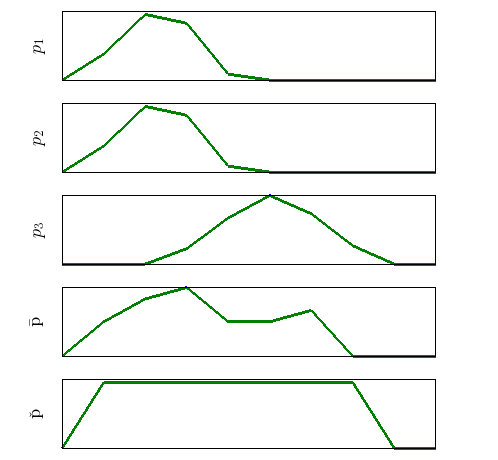
\includegraphics[width=0.9\linewidth]{./pic/prefsup102}
	  \end{center}
    \column{0.50\textwidth}
          \begin{center}
	      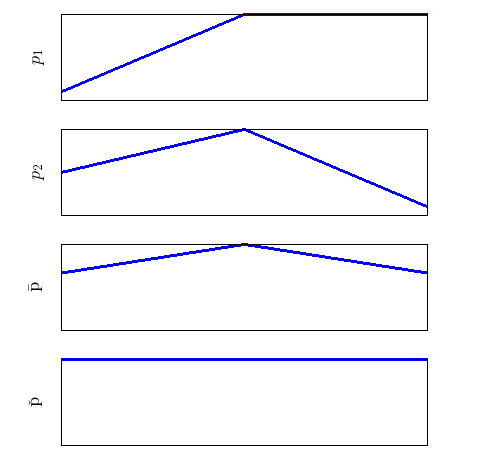
\includegraphics[width=1\linewidth]{./pic/prefsup6}
	  \end{center}
  \end{columns}
\end{frame} %===========================

\begin{frame}{Пример модели <<качества>> объекта}
	\begin{center}
		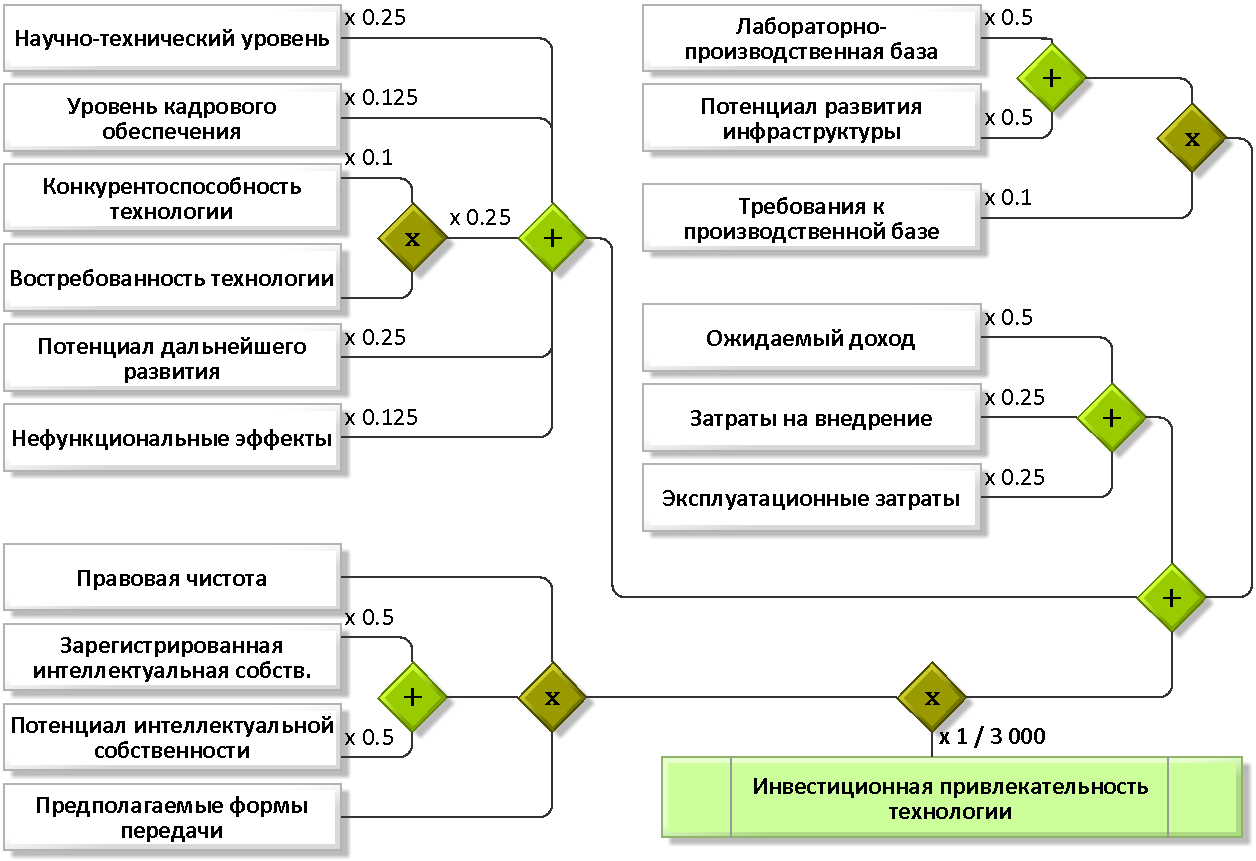
\includegraphics[width=0.85\linewidth]{./pic/schemeF2}
	\end{center}
\end{frame} %===========================

\begin{frame}{Примеры решений задачи выбора}
 \begin{center}
	\begin{columns}
	 \column{0.50\textwidth}  
	 \vspace{-1ex}
	 \begin{equation*}
	    n = 15, m = 16,  f: \text{см. блок-схему}.
	 \end{equation*}
	  \vspace{-4ex}
	  {
	      \\[0.5ex] \hspace{2ex} Для k=2  :  6 7; 
	      \\[0.5ex] \hspace{2ex} Для k=14:  все, кроме 13; 
	      \\[0.5ex] \hspace{2ex} Для остальных k -- неоднозначно.
	  }
	  \vspace{1ex}
	  \begin{center}
	    \resizebox{0.7\linewidth}{!}{\showevDisplayFullScale{./pic/realScaled13.txt}}
	  \end{center} 
	 \column{0.45\textwidth}
	  \begin{equation*}
	    \hspace{-2ex} n = 3, m = 1, f(x) = x.
	  \end{equation*}
	  \\ \vspace{1ex}
	      \resizebox{0.9\linewidth}{!}{\showevDisplay{./pic/sample1/ex1.txt}}
	      \\ \hspace{2ex} Ранжировка (Э1): $1, 2, 3$.
		  \\ \vspace{1ex}
	      \resizebox{0.9\linewidth}{!}{\showevDisplayRough{./pic/sample1/ex2.txt}}
	      \\ \hspace{2ex} Ранжировка (Э2): $3, 2, 1$.	      
		  \\ \vspace{1ex}
	      \resizebox{0.9\linewidth}{!}{\showevDisplayRough{./pic/sample1/mean.txt}}
	      \\ \hspace{2ex}  Ранжировка (среднее): $2, 3, 1$.
		  \\ \vspace{1ex}
	      \resizebox{0.9\linewidth}{!}{\showevDisplayRough{./pic/sample1/sup.txt}}
	      \\ \hspace{2ex} Ранжировка (супремум): \textbf{?}	     
	
	\end{columns}
 \end{center}
\end{frame} %===========================

\begin{frame}{Пользовательский интерфейс}
          \begin{center}
	      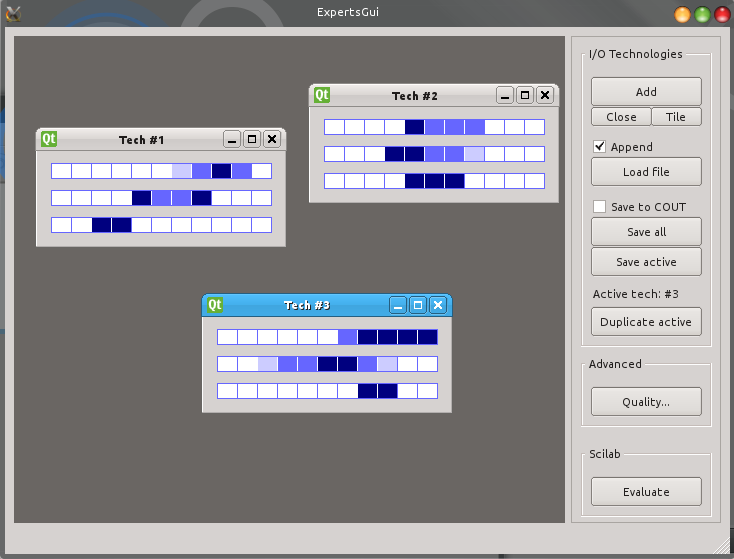
\includegraphics[width=0.75\linewidth]{./pic/combination6}
	  \end{center}
\end{frame} %===========================
% == eof == eof ===
